%% BioMed_Central_Tex_Template_v1.06
%%                                      %
%  bmc_article.tex            ver: 1.06 %
%                                       %

%%IMPORTANT: do not delete the first line of this template
%%It must be present to enable the BMC Submission system to
%%recognize this template!!

%%%%%%%%%%%%%%%%%%%%%%%%%%%%%%%%%%%%%%%%%
%%                                     %%
%%  LaTeX template for BioMed Central  %%
%%     journal article submissions     %%
%%                                     %%
%%          <8 June 2012>              %%
%%                                     %%
%%                                     %%
%%%%%%%%%%%%%%%%%%%%%%%%%%%%%%%%%%%%%%%%%


%%%%%%%%%%%%%%%%%%%%%%%%%%%%%%%%%%%%%%%%%%%%%%%%%%%%%%%%%%%%%%%%%%%%%
%%                                                                 %%
%% For instructions on how to fill out this Tex template           %%
%% document please refer to Readme.html and the instructions for   %%
%% authors page on the biomed central website                      %%
%% http://www.biomedcentral.com/info/authors/                      %%
%%                                                                 %%
%% Please do not use \input{...} to include other tex files.       %%
%% Submit your LaTeX manuscript as one .tex document.              %%
%%                                                                 %%
%% All additional figures and files should be attached             %%
%% separately and not embedded in the \TeX\ document itself.       %%
%%                                                                 %%
%% BioMed Central currently use the MikTex distribution of         %%
%% TeX for Windows) of TeX and LaTeX.  This is available from      %%
%% http://www.miktex.org                                           %%
%%                                                                 %%
%%%%%%%%%%%%%%%%%%%%%%%%%%%%%%%%%%%%%%%%%%%%%%%%%%%%%%%%%%%%%%%%%%%%%

%%% additional documentclass options:
%  [doublespacing]
%  [linenumbers]   - put the line numbers on margins

%%% loading packages, author definitions

%\documentclass[twocolumn]{bmcart}% uncomment this for twocolumn layout and comment line below
\documentclass{bmcart}

%%% Load packages
\usepackage{amsthm,amsmath}
%\RequirePackage{natbib}
%\RequirePackage{hyperref}
\usepackage[utf8]{inputenc} %unicode support
%\usepackage[applemac]{inputenc} %applemac support if unicode package fails
%\usepackage[latin1]{inputenc} %UNIX support if unicode package fails
\usepackage{graphicx}

%%%%%%%%%%%%%%%%%%%%%%%%%%%%%%%%%%%%%%%%%%%%%%%%%
%%                                             %%
%%  If you wish to display your graphics for   %%
%%  your own use using includegraphic or       %%
%%  includegraphics, then comment out the      %%
%%  following two lines of code.               %%
%%  NB: These line *must* be included when     %%
%%  submitting to BMC.                         %%
%%  All figure files must be submitted as      %%
%%  separate graphics through the BMC          %%
%%  submission process, not included in the    %%
%%  submitted article.                         %%
%%                                             %%
%%%%%%%%%%%%%%%%%%%%%%%%%%%%%%%%%%%%%%%%%%%%%%%%%


%\def\includegraphic{}
%\def\includegraphics{}



%%% Put your definitions there:
\startlocaldefs
\endlocaldefs


%%% Begin ...
\begin{document}

%%% Start of article front matter
\begin{frontmatter}

\begin{fmbox}
\dochead{Review}

%%%%%%%%%%%%%%%%%%%%%%%%%%%%%%%%%%%%%%%%%%%%%%
%%                                          %%
%% Enter the title of your article here     %%
%%                                          %%
%%%%%%%%%%%%%%%%%%%%%%%%%%%%%%%%%%%%%%%%%%%%%%

\title{Image Processing for Optical Mapping}

%%%%%%%%%%%%%%%%%%%%%%%%%%%%%%%%%%%%%%%%%%%%%%
%%                                          %%
%% Enter the authors here                   %%
%%                                          %%
%% Specify information, if available,       %%
%% in the form:                             %%
%%   <key>={<id1>,<id2>}                    %%
%%   <key>=                                 %%
%% Comment or delete the keys which are     %%
%% not used. Repeat \author command as much %%
%% as required.                             %%
%%                                          %%
%%%%%%%%%%%%%%%%%%%%%%%%%%%%%%%%%%%%%%%%%%%%%%

\author[
   addressref={aff1},                   % id's of addresses, e.g. {aff1,aff2}
   corref={aff1},                       % id of corresponding address, if any
%   noteref={n1},                        % id's of article notes, if any
   email={pravindran@wisc.edu}   % email address
]{\inits{PR}\fnm{Prabu} \snm{Ravindran}}

\author[
   addressref={aff1},
   email={agupta29@wisc.edu}
]{\inits{AG}\fnm{Aditya} \snm{Gupta}}

%%%%%%%%%%%%%%%%%%%%%%%%%%%%%%%%%%%%%%%%%%%%%%
%%                                          %%
%% Enter the authors' addresses here        %%
%%                                          %%
%% Repeat \address commands as much as      %%
%% required.                                %%
%%                                          %%
%%%%%%%%%%%%%%%%%%%%%%%%%%%%%%%%%%%%%%%%%%%%%%

\address[id=aff1]{%                           % unique id
  \orgname{Laboratory for Molecular and Computational Genomics, University of Wisconsin}, % university, etc
  \street{425 Henry Mall},                     %
  %\postcode{}                                % post or zip code
  \city{Madison},                              % city
  \cny{USA}                                    % country
}
%\address[id=aff2]{%
%  \orgname{Marine Ecology Department, Institute of Marine Sciences Kiel},
%  \street{D\"{u}sternbrooker Weg 20},
%  \postcode{24105}
%  \city{Kiel},
%  \cny{Germany}
%}

%%%%%%%%%%%%%%%%%%%%%%%%%%%%%%%%%%%%%%%%%%%%%%
%%                                          %%
%% Enter short notes here                   %%
%%                                          %%
%% Short notes will be after addresses      %%
%% on first page.                           %%
%%                                          %%
%%%%%%%%%%%%%%%%%%%%%%%%%%%%%%%%%%%%%%%%%%%%%%

\begin{artnotes}
%\note{Sample of title note}     % note to the article
%\note[id=n1]{Equal contributor} % note, connected to author
\end{artnotes}

\end{fmbox}% comment this for two column layout

%%%%%%%%%%%%%%%%%%%%%%%%%%%%%%%%%%%%%%%%%%%%%%
%%                                          %%
%% The Abstract begins here                 %%
%%                                          %%
%% Please refer to the Instructions for     %%
%% authors on http://www.biomedcentral.com  %%
%% and include the section headings         %%
%% accordingly for your article type.       %%
%%                                          %%
%%%%%%%%%%%%%%%%%%%%%%%%%%%%%%%%%%%%%%%%%%%%%%

\begin{abstractbox}

\begin{abstract} % abstract
Optical Mapping is an established single-molecule, whole-genome analysis system, 
which has been used to gain a comprehensive understanding of genomic structure 
and to study structural variation of complex genomes. A critical component of 
Optical Mapping system is the image processing module, which extracts single 
molecule restriction maps from image datasets of immobilized, restriction 
digested and fluorescently stained large DNA molecules. In this review, we 
describe robust and efficient image processing techniques to process these 
massive datasets and extract accurate restriction maps in the presence of noise, ambiguity and confounding artifacts. We also highlight a few applications of the Optical Mapping system. 


%\parttitle{First part title} %if any
%Text for this section.

%\parttitle{Second part title} %if any
%Text for this section.
\end{abstract}

%%%%%%%%%%%%%%%%%%%%%%%%%%%%%%%%%%%%%%%%%%%%%%
%%                                          %%
%% The keywords begin here                  %%
%%                                          %%
%% Put each keyword in separate \kwd{}.     %%
%%                                          %%
%%%%%%%%%%%%%%%%%%%%%%%%%%%%%%%%%%%%%%%%%%%%%%

\begin{keyword}
\kwd{Optical Mapping}
\kwd{Image processing}
\kwd{Skeletonization}
\kwd{Grouping}
\kwd{Tiling}
\kwd{Shortest path}
\kwd{Integrated fluorescence intensity}
\end{keyword}

% MSC classifications codes, if any
%\begin{keyword}[class=AMS]
%\kwd[Primary ]{}
%\kwd{}
%\kwd[; secondary ]{}
%\end{keyword}

\end{abstractbox}
%
%\end{fmbox}% uncomment this for twcolumn layout

\end{frontmatter}

%%%%%%%%%%%%%%%%%%%%%%%%%%%%%%%%%%%%%%%%%%%%%%
%%                                          %%
%% The Main Body begins here                %%
%%                                          %%
%% Please refer to the instructions for     %%
%% authors on:                              %%
%% http://www.biomedcentral.com/info/authors%%
%% and include the section headings         %%
%% accordingly for your article type.       %%
%%                                          %%
%% See the Results and Discussion section   %%
%% for details on how to create sub-sections%%
%%                                          %%
%% use \cite{...} to cite references        %%
%%  \cite{koon} and                         %%
%%  \cite{oreg,khar,zvai,xjon,schn,pond}    %%
%%  \nocite{smith,marg,hunn,advi,koha,mouse}%%
%%                                          %%
%%%%%%%%%%%%%%%%%%%%%%%%%%%%%%%%%%%%%%%%%%%%%%

%%%%%%%%%%%%%%%%%%%%%%%%% start of article main body
% <put your article body there>

%%%%%%%%%%%%%%%%
%% Background %%
%%
\section*{Introduction}
Optical Mapping~\cite{Schwartz1993, Dimalanta2004, Teague2010} is a 
high-throughput, single-molecule system that generates ordered restriction 
maps (also called Rmaps) from high molecular weight genomic 
DNA molecules, ranging in size from 300 kilobases to megabases. The Rmaps are 
then used for the construction of genome-wide physical restriction maps using computational approaches, which provide insights into long range genome 
structure and genome variation. It is made possible by the integration of many 
diverse components that draw from surface chemistry, microfluidics, fluorescence microscopy, image processing and other computational approaches. The mapping 
system uses unamplified genomic DNA as substrate, thereby yielding a view of the genome free of cloning or amplification biases.

%~\cite{Schwartz1993, Meng1995, 
%Cai1995, Anantharaman1997, Cai1998, Jing1998, Anantharaman1999, Skiadas1999, 
%Lai1999, Lin1999, Lim2001, Perna2001, Zhou2003, Zhou2004, Dimalanta2004, 
%Valouev2006a, Valouev2006b, Valouev2006c, Zhou2007, Kidd2008, Zhou2009, 
%Antonacci2010, Teague2010, Chen2012, Ray2013}.

An outline of Optical Mapping is provided in Fig. 1. Here, we provide a brief description of the system. The first step in Optical Mapping is DNA extraction. Because high molecular weight DNA is required as a substrate, very gentle DNA extraction methods like liquid lysis of cell suspensions or preparation of DNA 
inserts~\cite{Schwartz1984} are commonly used. Next, DNA is presented on 
glass cover slips that are acid cleaned and derivatized with a mixture of aminosilanes. The derivatization process imparts a positive charge to glass 
surfaces, which allows DNA immobilization~\cite{Meng1995, Cai1995, Hu1997, 
Lim2001}. DNA presentation is accomplished \emph{via} capillary flow 
in microchannels, which are formed at the interface of derivatized glass 
surfaces adhered to a microfluidic device fabricated using soft lithography 
approaches~\cite{Dimalanta2004}. Use of a microfluidic device allows for 
massively-parallel, high throughput deposition of single DNA molecules on 
derivatized glass surfaces. DNA presentation accomplishes two goals: elongation 
and immobilization. DNA elongation allows the imaging of molecular cleavage 
events once intact DNA molecules are digested using restriction endonucleases, 
and is an important requirement for generation of Rmaps. DNA immobilization 
serves to fix DNA in place, which is important to ensure that i) the linear 
order of DNA fragments from each DNA molecule is preserved; ii) the digested 
molecules can be imaged easily; and iii) the fragments generated after 
restriction digestion do not desorb and get lost before imaging. Both these 
steps, elongation and immobilization, are carefully controlled to ensure that 
the biochemical action of restriction endonucleases is preserved and that the 
DNA molecules are optimally stretched out to be able to generate useful Rmap 
data. Following presentation, the DNA molecules are digested with a restriction endonuclease of choice. Upon digestion, the double-stranded DNA digestion sites present as gaps that are formed between fragments due to DNA relaxation at cut 
ends~\cite{Schwartz1993, Meng1995}. Next, digested DNA is stained 
using intercalating fluorochrome YOYO-1~\cite{Cai1995} and imaged using 
automated laser-illuminated epifluorescence microscopy 
systems~\cite{Dimalanta2004, Jing1998, Skiadas1999, Zhou2004}. Custom in-house software allows automated imaging of an entire array of microchannels with very 
little setup time. Once the images have been collected, they are automatically processed using custom image processing software to generate Rmaps, which are 
obtained as ordered series of fragment sizes derived from digested single DNA 
molecules~\cite{Dimalanta2004, Teague2010}. Once a large dataset of Rmaps has 
been collected using the Optical Mapping system, a computational pipeline that 
uses Bayesian inference approaches~\cite{Anantharaman1999} and cluster 
computing is used to assemble the Rmaps into genome-wide contigs and generate 
genome-wide consensus 
maps~\cite{Teague2010, Valouev2006a, Valouev2006b, Valouev2006c}. The image 
processing module is an important contributor to successful implementation of 
Optical Mapping, and is the central focus of this review.


\section*{Image Processing Methodology}
The goal of the image processing module is to accurately and robustly extract 
the Rmaps data from image datasets. An image processing module for 
Optical Mapping must provide the following capabilities:
\begin{itemize}
\item
Skeletonization: The single pixel centerline for each fragment is detected as a 
column ordered connected component or skeletal segment.
\item
Tiling: A single Rmap can span multiple images. In order to extract multi-frame 
Rmaps, a mosaic of images acquired from a single microchannel is created by 
aligning adjacent images using the skeletal segments.
\item
Grouping: The skeletal segments are grouped such that each group corresponds to 
fragments from the same DNA molecule.
\item
Sizing: Groups of skeletal segments that correspond to standards are 
detected; conversion factors for these skeletal segments are computed 
using integrated fluorescence intensity and the known size of fragments for the standards. The estimated conversion factor is applied to construct Rmaps (in 
kilobases) for genomic DNA molecules.         
\end{itemize}
Different versions of image processing software for Optical Mapping have been implemented over the last two decades. During the early days of Optical Mapping 
useful map data was obtained using completely manual methods for detecting and 
sizing the fragments. Improvements to the image acquisition~\cite{Jing1998} and 
image processing software~\cite{Skiadas1999} culminated in the development of 
the semi-automatic Autovis system~\cite{Lim2001}. PathFinder~\cite{Dimalanta2004, Zhou2004} was the first fully featured, automated image processing system 
developed for Optical Mapping and was instrumental is making large scale Optical Mapping projects feasible. The image processing methodology detailed below is 
inspired by the techniques implemented in the PathFinder system.         

\subsection*{Skeletonization}
The first step extracts skeletal segments that correspond to the digestion 
induced fragments of DNA molecules. An image pixel $I(r, c)$ is a 
skeletal pixel if \emph{all} of the following conditions are satisfied:
\begin{align}
I(r, c)~&\geq~I(r - 1, c) \label{eq:skel_cond1}\\
I(r, c)~&\geq~I(r + 1, c) \label{eq:skel_cond2}\\
I(r, c) - I(r - 2, c)~&>~\delta_f \label{eq:skel_cond3}\\ 
I(r, c) - I(r + 2, c)~&>~\delta_f \label{eq:skel_cond4},
\end{align}
where $I(r, c)$ represents the image intensity at pixel $(r, c)$ and $\delta_f$ 
is an user specified threshold that denotes expected falloff 
in intensity grey levels over two pixels. The local neighborhood used for the 
computation is shown in figure~\ref{fig:skel}(a). The above constraints and 
geometry for the neighborhood are based on the facts that (i) the DNA molecules 
are deposited along the direction of flow in microchannels and (ii) the ideal fluorescence intensity profile falls off rapidly from the peak intensity, 
perpendicular to the deposited molecules. This physically motivated local 
computation results in an intuitive, efficient and robust direct gray scale skeletonization technique.   

While the $\geq$ sign in equations~\ref{eq:skel_cond1} 
and~\ref{eq:skel_cond2} maintains connectedness of the skeletal pixels in a 
segment, it may also produce skeletons that are not one pixel wide. Hence, for 
each segment, the one pixel wide skeleton is extracted as the shortest path 
between the segment end points using Dijkstra's algorithm~\cite{Cormen2009}. 
The accurate localization of end points is aided by the increased intensity 
pixels due to coil relaxation at enzyme cleavage sites. An example extracted 
skeleton with end points is shown in figure~\ref{fig:skel}(c).  

\subsection*{Tiling}
The image acquisition system captures multiple overlapping images along each 
microchannel. Accordingly, long DNA molecules that span several frames are 
imaged, which necessitates tiling. As a linear stage is employed to acquire 
overlapping images, the geometric transformation that is used to model 
the tiling of adjacent images is a translation. 
 
The translation between adjacent frames is estimated using the left and right 
end points of the extracted skeletal segments as landmarks. Given two adjacent 
images, the translation that matches the maximum subset of landmarks from one 
image to the other is taken as the tiling transformation. As the amount of 
overlap between images is engineered into the acquisition process (typically 
$25$~percent), search for the tiling translation is localized to a small 
range of values. Having the tiling information between pairs of images is 
required to extract Rmaps that span multiple images. It is not required to 
explicitly create a single mosaic of the entire channel (see 
figure~\ref{fig:tile}).  
      
\subsection*{Grouping}
Skeletal segments that come from the same DNA molecule are incrementally 
grouped and column ordered using spatial proximity of skeletal segment end 
points and directional agreement with respect to fluid flow based deposition. 
Specifically, the grouping constraints are:
\begin{itemize}
\item A skeletal segment can belong to utmost one group.
\item Adjacent skeletal segments in the same group have no overlap.
\item For segments $S_l$ and $S_r$, the ordered grouping $(S_l, S_r)$ is valid 
if $S_r$ is the best segment to pair with $S_l$ when ``growing" $S_l$ on its 
right \emph{and} vice versa. When determining the best segment both spatial 
proximity and orientational similarity of the segments (\emph{via} straight 
line fits) are used.    
\end{itemize}
The constraints and examples of grouping in the presence of distracting 
artifacts are depicted in figure~\ref{fig:group}.

\subsection*{Sizing}
The two main factors that influence fragment sizing are: (i) intensity 
fluctuations due to local variations in the elongation of the DNA molecule or staining, and (ii) increased intensity regions adjacent to enzyme cleavage 
sites due to coil relaxation. Fragment sizes obtained using integrated 
fluorescence values are robust to these local effects. In order to convert the 
integrated fluorescence values into kilobases, standards are used to used to 
estimate the conversion factor.

With the skeletal segments grouped, groups that correspond to the standards 
are identified based on the expected number of fragments and their relative 
lengths. A mask that extends for two pixels on either side of 
the skeletal pixels is created and the fluorescence intensities in this region 
are summed to yield the integrated fluorescence values. The conversion factor 
$C_{kb}$ that maps the integrated fluorescence values into kilobases is 
estimated (using the fragments of the standards) as the ratio:
\begin{equation}
C_{kb} = \frac{\mbox{size of fragment in kilobases}}
              {\mbox{integrated fluorescence value of fragment}}.
\end{equation} 
The estimated $C_{kb}$ is used to construct Rmaps from groups of ordered 
skeletal segments by converting integrated fluorescence values (computed using 
the same masks used for the standards) to kilobases (figure~\ref{fig:size}). 


\section*{Applications}
Fully automated image processing allowed for rapid analysis of DNA molecules 
deposited in microchannels, which helped understand key physical 
characteristics of the deposition process (such as DNA elongation and 
deposition density along the microchannel) and design optimal operating parameters 
for Optical Mapping~\cite{Dimalanta2004}. This enabled the generation of 
massive Rmap datasets, which facilitated high resolution analysis of genomes 
of various sizes.
   
Rmap assemblies provide long range structural information about the genome. Consequently, they generate a scaffold that can be used to verify or guide DNA sequencing based genome assemblies. Optical Mapping was first used to verify sequencing based chromosomal~\cite{Jing1999} and genome 
assemblies~\cite{Lin1999}. With an increase in throughput, it was used to 
generate physical assemblies to aid sequencing based genome assembly for many microbial genomes. These include some bacterial genomes like \emph{Deinococcus 
radiodurans}~\cite{Lin1999}, \emph{Escherichia coli} O157:H7~\cite{Lim2001}, 
\emph{Yersinia pestis}~\cite{Zhou2002} and \emph{Rhodobacter 
sphaeroides} 2.4.1~\cite{Zhou2003}. By comparing different bacterial strains to identify genomic differences, Optical Mapping was used for comparative 
genomics~\cite{Zhou2004}. More recently, plant genomes like 
rice~\cite{Zhou2007} and maize~\cite{Zhou2009, Wei2009} and 
normal~\cite{Teague2010} and cancer~\cite{Ray2013} human genomes have 
been mapped. These assemblies have helped in validation of sequencing based 
assemblies and have also provided high-resolution scaffolds for gap closure 
and for correcting sequencing based assembly errors~\cite{Reslewic2005}. 

Optical Mapping of human genomes has uncovered a wide array of structural 
variation in these genomes. Teague et al. identified thousands of structural 
variants, ranging in size from a few kilobases to megabases in a complete 
hydatidiform mole and three lymphoblast-derived cell 
lines~\cite{Teague2010}. The authors also identified many structural 
variants that were inaccessible to other genomic analysis platforms. Later, 
Ray et al. studied tumor genomes from two oligodendroglioma patient samples, 
the first use of Optical Mapping to study a solid tumor genome, to reveal 
many somatic structural variants and copy number heterogeneity~\cite{Ray2013}.

\section*{Conclusions}
The successful implementation of the automated image processing techniques 
described in this review has allowed the high resolution analysis of many 
complex genomes. It has also enabled the study of the physical characteristics 
of DNA deposition using microfuidic systems. In addition variants of the image processing techiques described in this review have been incorporated into the Nanocoding system, a higher resolution and more accurate successor to 
Optical Mapping~\cite{Jo2007, Pag2013}.  


%%%%%%%%%%%%%%%%%%%%%%%%%%%%%%%%%%%%%%%%%%%%%%
%%                                          %%
%% Backmatter begins here                   %%
%%                                          %%
%%%%%%%%%%%%%%%%%%%%%%%%%%%%%%%%%%%%%%%%%%%%%%

\begin{backmatter}

\section*{Competing interests}
  The authors declare that they have no competing interests.

\section*{Author's contributions}
 The authors contributed equally to the manuscript. 

\section*{Acknowledgements}
We would like to thank Prof. David C. Schwartz for his invaluable insights, 
support and guidance during the writing of this review. We would also like to acknowledge Konstantinos Potamousis, Michael Place, Steve Goldstein, 
Shiguo Zhou and Michael Bechner for helpful discussions and feedback. PR and AG 
would like to thank NHGRI for support (R01HG000225).   
%%%%%%%%%%%%%%%%%%%%%%%%%%%%%%%%%%%%%%%%%%%%%%%%%%%%%%%%%%%%%
%%                  The Bibliography                       %%
%%                                                         %%
%%  Bmc_mathpys.bst  will be used to                       %%
%%  create a .BBL file for submission.                     %%
%%  After submission of the .TEX file,                     %%
%%  you will be prompted to submit your .BBL file.         %%
%%                                                         %%
%%                                                         %%
%%  Note that the displayed Bibliography will not          %%
%%  necessarily be rendered by Latex exactly as specified  %%
%%  in the online Instructions for Authors.                %%
%%                                                         %%
%%%%%%%%%%%%%%%%%%%%%%%%%%%%%%%%%%%%%%%%%%%%%%%%%%%%%%%%%%%%%

% if your bibliography is in bibtex format, use those commands:
\bibliographystyle{bmc-mathphys} % Style BST file
\bibliography{gigascience_submit}      % Bibliography file (usually '*.bib' )
%\bibliography{bmc_article}      % Bibliography file (usually '*.bib' )

% or include bibliography directly:
% \begin{thebibliography}
% \bibitem{b1}
% \end{thebibliography}

%%%%%%%%%%%%%%%%%%%%%%%%%%%%%%%%%%%
%%                               %%
%% Figures                       %%
%%                               %%
%% NB: this is for captions and  %%
%% Titles. All graphics must be  %%
%% submitted separately and NOT  %%
%% included in the Tex document  %%
%%                               %%
%%%%%%%%%%%%%%%%%%%%%%%%%%%%%%%%%%%

%%
%% Do not use \listoffigures as most will included as separate files

\section*{Figures}
\begin{figure}[h!]
\centering
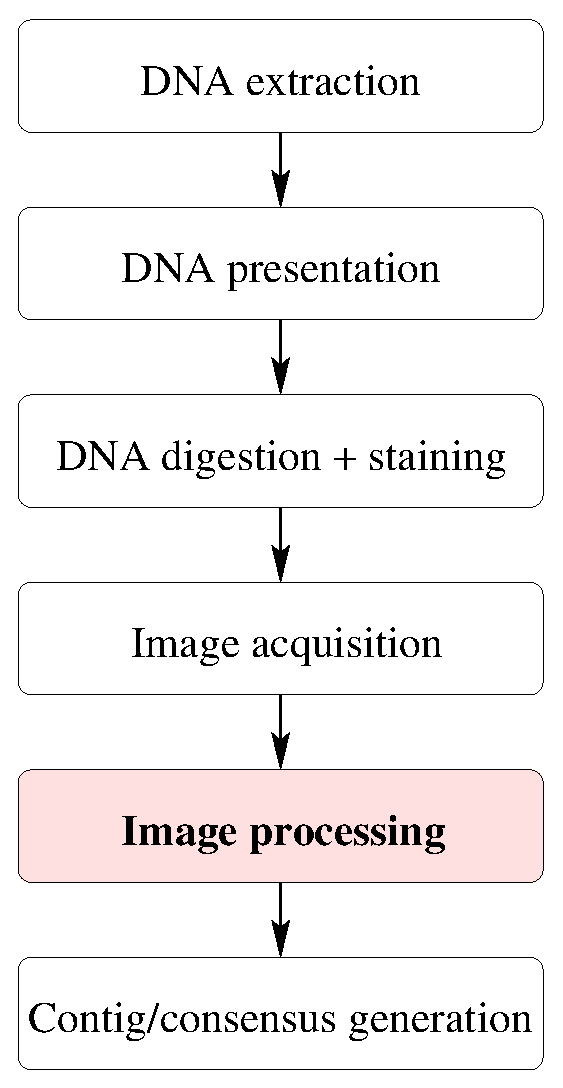
\includegraphics[width=0.9\linewidth]{optical_mapping_pipeline}
\caption{\csentence{Schematic of Optical Mapping.}
The various steps in the Optical Mapping system. This review describes 
the image processing methodology and highlights some of the applications.}
\label{fig:om}
\end{figure}

\begin{figure}[h!]
\centering
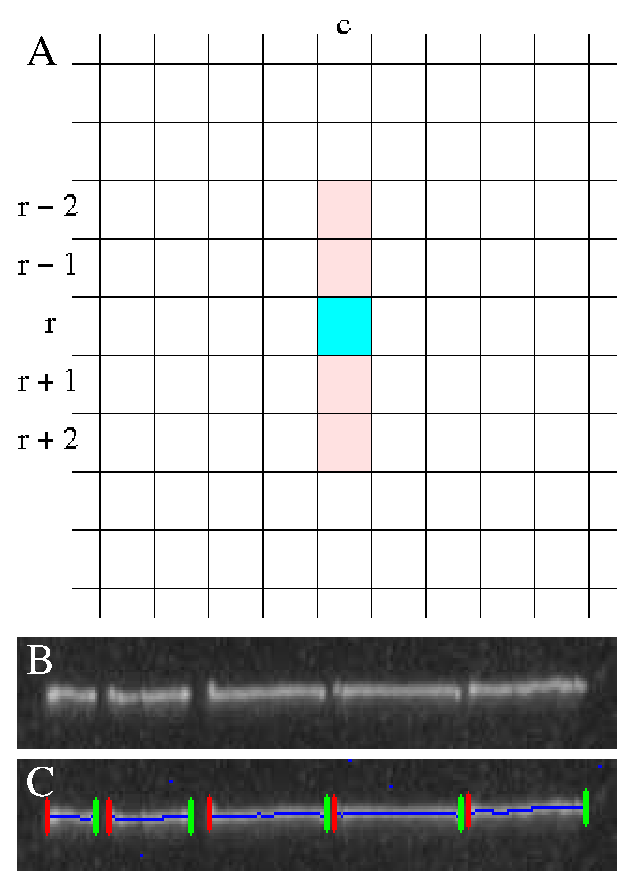
\includegraphics[width=0.9\linewidth]{skeleton_figure}
\caption{\csentence{Skeletonization.}
(A) The local neighborhood in which the inequality 
constraints~(\ref{eq:skel_cond1})-(\ref{eq:skel_cond4}) are applied to detect 
skeletal pixels. (B) An example image patch. (C) Extracted skeleton in the 
example image patch. Skeletal pixels are shown in blue. Red and green lines 
represent the left and right endpoints of each skeletal segment.}
\label{fig:skel}
\end{figure}

\begin{figure}[h!]
\centering
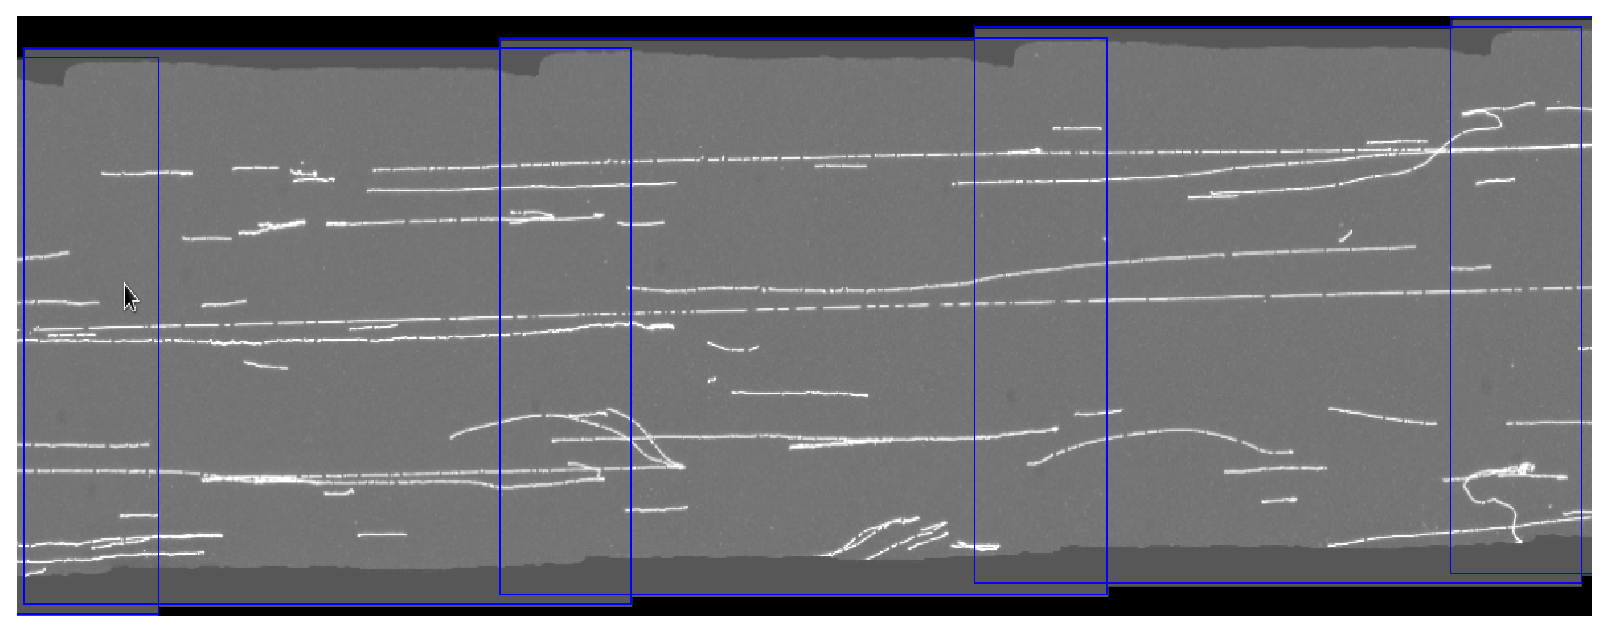
\includegraphics[width=0.95\textwidth]{tiling_example}
\caption{\csentence{Tiling.}
Example of tiling three images from a microchannel. A horizontal span of about 
$140$ microns is covered by each image. The blue outlines represent the image 
borders. The estimated tiling transformation provides the translation 
of frames to achieve this seamless mosaic, but the mosaic itself is not 
explicitly constructed. Estimating the tiling transformation is required to 
extract multi-frame Rmaps.}
\label{fig:tile}
\end{figure}

\begin{figure*}[h!]
\centering
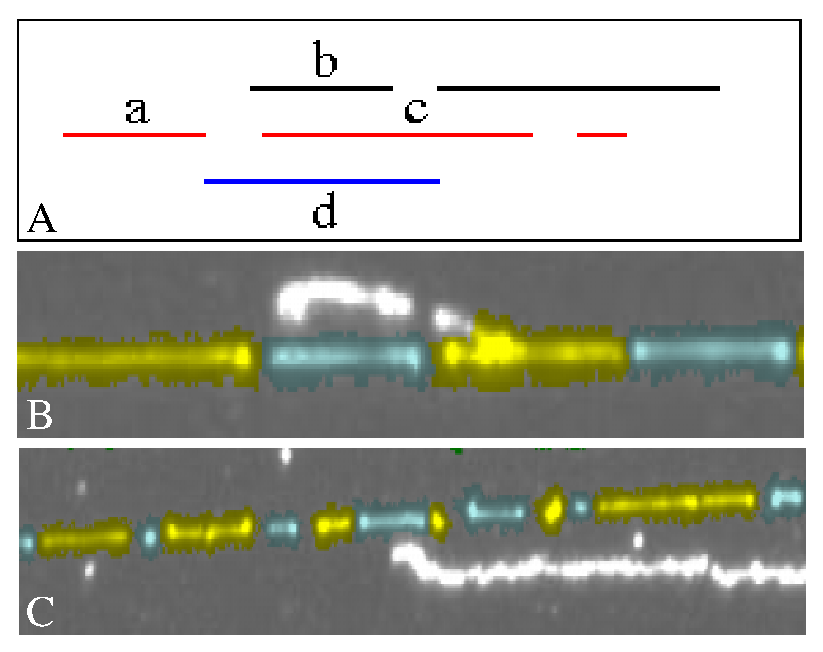
\includegraphics[width=0.8\linewidth]{grouping_figure}
\caption{\csentence{Grouping.}
(A) Segments $a$ and $c$ are grouped as this grouping provides the best 
continuity in terms of adhering to the constraints of spatial proximity and 
orientation similarity. The grouping $(a, b)$ satisfies the spatial proximity constraint but in terms of orientation similarity, it is less optimal that the 
grouping $(a, c)$. The grouping $(a, d)$ is invalid as we require the segment 
$d$ to be strictly non-overlapping with segment $a$. (B), (C) Two examples 
of accurate grouping in the presence of distractors. The adjacent fragments are colored differently to aid 
visualization.}
\label{fig:group}
\end{figure*}

\begin{figure}[h!]
\centering
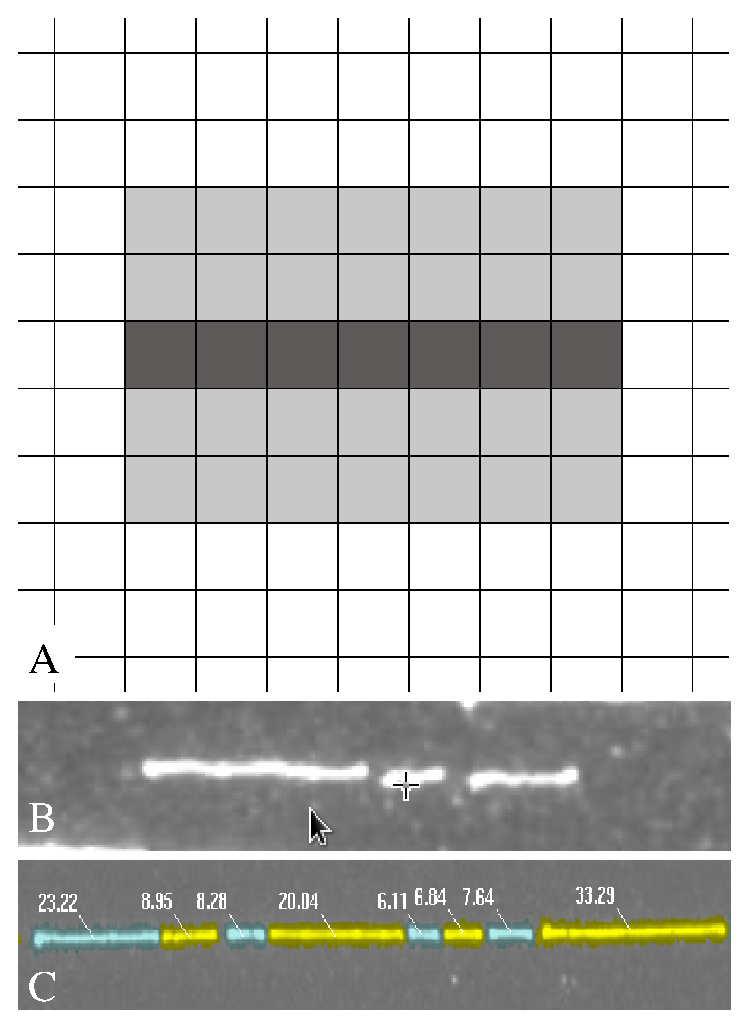
\includegraphics[width=0.8\linewidth]{sizing_figure}
\caption{\csentence{Sizing.}
(A) The two pixel wide mask used to compute the integrated fluorescence 
values for fragments. The darker grey pixels represent the skeletal pixels. 
Shown here is a fragment that spans $7$ pixels. (B) An example three fragment, 
Bsu36I digested, Lambda DNA standard ($\approx 48.5$kb) used to estimate 
$C_{kb}$. The expected fragment sizes (in kilobases) are: $26.718$, $7.601$ 
and $14.183$. Standards can be selected based on the experiment. (C) A portion 
of a Rmap with fragment sizes using the estimated $C_{kb}$ to determine sizes 
in kilobases from integrated fluorescence values.}
\label{fig:size}
\end{figure}

%%%%%%%%%%%%%%%%%%%%%%%%%%%%%%%%%%%
%%                               %%
%% Tables                        %%
%%                               %%
%%%%%%%%%%%%%%%%%%%%%%%%%%%%%%%%%%%

%% Use of \listoftables is discouraged.
%%
%\section*{Tables}
%\begin{table}[h!]
%\caption{Sample table title. This is where the description of the table should go.}
%      \begin{tabular}{cccc}
%        \hline
%           & B1  &B2   & B3\\ \hline
%        A1 & 0.1 & 0.2 & 0.3\\
%        A2 & ... & ..  & .\\
%        A3 & ..  & .   & .\\ \hline
%      \end{tabular}
%\end{table}

%%%%%%%%%%%%%%%%%%%%%%%%%%%%%%%%%%%
%%                               %%
%% Additional Files              %%
%%                               %%
%%%%%%%%%%%%%%%%%%%%%%%%%%%%%%%%%%%

%\section*{Additional Files}
%  \subsection*{Additional file 1 --- Sample additional file title}
%    Additional file descriptions text (including details of how to
%    view the file, if it is in a non-standard format or the file extension).  This %might
%    refer to a multi-page table or a figure.

%  \subsection*{Additional file 2 --- Sample additional file title}
%    Additional file descriptions text.


\end{backmatter}
\end{document}


